\documentclass[11pt]{article}
\usepackage{graphicx}
\usepackage[font=footnotesize, labelfont={sf,bf}, margin=1cm]{caption}
\usepackage{mathtools}
\usepackage{wrapfig}
\usepackage[letterpaper, portrait, margin=1in]{geometry}
\usepackage{framed}
\usepackage{listings}
\usepackage{color}
\usepackage{float}
\usepackage[utf8]{inputenc}
\lstset{frame=tb,
  language=Lisp,
  aboveskip=3mm,
  belowskip=3mm,
  showstringspaces=false,
  columns=flexible,
  basicstyle={\small\ttfamily},
  numbers=none,
  numberstyle=\tiny\color{gray},
  keywordstyle=\color{blue},
  commentstyle=\color{cyan},
  stringstyle=\color{mauve},
  breaklines=true,
  breakatwhitespace=true,
  tabsize=3
}
%Gummi|065|=)
\title{\textbf{How can I implement Grover's algorithm based on a quantum computation simulator in Scheme?}}
\author{William Bernoudy}
\date{}
\begin{document}

\maketitle

\begin{abstract}
I explain the basics of quantum computing, the quantum computation simulator I wrote using Scheme, and how Grover's algorithm could be implemented on a quantum computer. I then present a method of designing a oracle from a given classical circuit representing the search function.
\end{abstract}
\section{Introduction}

\subsection{Context}

With the current state of computer technology and the internet, humans generate more data now than ever before. Of course, to be useful, this information must be stored in databases. For many applications, data cannot be entered into the database in an ordered way. This means data entries are simply entered as they come. However, for this information to remain useful, there must be a way of searching the database to look for desired entries. Currently, the most effective way to do this simply means going through every entry until one is found that matches the desired quality. In other words, the best algorithm has a time complexity of $O(n)$, with an average of $\frac{n}{2}$.

In 1996, Lov Grover published a paper outlining an entirely new method for searching databases \cite{grover96}. Called Grover's algorithm, it runs in $O(\sqrt{n})$ as opposed to $O(n)$ time, a significant speedup for large databases. To achieve this speedup, Grover's algorithm is designed to run on a quantum computer instead of on a classical one. This means that at the moment, there is no way to actually run Grover's algorithm and take advantage of the speedup, because quantum computers of sufficient qubits do not exist.

Despite the current state of quantum computation technology, researchers have already begun work on developing code for quantum computers. Because there are no elements of a quantum computer that cannot be simulated by a classical computer (everything just runs much more slowly), we don't have to wait until the technology catches up to work on implementing quantum algorithms. In fact, Lisp, a programming language developed in the 1950's, is ideal for expressing quantum algorithms. Lisp is based heavily in Lambda calculus, which is a simple and universal system for expressing computation. Lambda calculus uses only function definitions and variable substitution for the entirety of the system, and all computations consist only of those two things \cite{rojas04}. Since quantum computation can be formulated as a Lambda calculus, Lisp makes for a very natural medium \cite{tonder04}.

As databases are completely ubiquitous on the internet, with every sizable service requiring large databases, shortening the length of time needed to make a query will be hugely useful. Grover's algorithm provides a quadratic speedup for these queries. Furthermore, the applications of Grover's algorithm are not limited to searching databases stored on servers. It can also be used to find a solution to problem where an answer is easily verifiable. For example, while the best know classical algorithm for solving the 3-SAT problem is of time complexity $O(2^{n})$, Grover's algorithm can be used to reduce this to $O(2^{n/2})$. Because of the speedups it provides as well as its wide applicability, an implementation of Grover's algorithm will be very useful for the world.

\section{Analysis}

\subsection{How a quantum computer works}
(borrowed and modified from my Question Proposal)

A quantum computer is a computer that takes advantage of quantum phenomena. Specifically, it is a computer based on qubits instead of bits. Qubits are peices of information that interact in ways not possible with a classical understanding. For example, unlike a classical bit, a qubit can be in a superposition of multiple states at once.

Let’s say we have one qubit called $\psi$. Its vector is given by:
$$ \left | \psi \right \rangle=\alpha _{0}\left | 0 \right \rangle+\alpha _{1}\left | 1 \right \rangle=\begin{pmatrix}\alpha_{0}\\ \alpha_{1}\end{pmatrix}$$
where  and  are complex numbers under the single constraint 
$$ \left | \alpha_{0} \right |^{2} + \left | \alpha_{1} \right |^{2}=1$$
This means that the  values have an infinite number of possibilities. Unlike a classical bit, for which the vector could only consist of all zeroes and one “1”, there are an infinite number of directions $\psi$ can be pointing. This is a mathematical way of saying that $\psi$ is not really in either the $\left | 0 \right \rangle$ state or the $\left | 1 \right \rangle$ state, but in a superposition of both. It exists as some amount of both at the same time.

\begin{wrapfigure}{l}{0.5\textwidth}
    \begin{center}
    \def\svgwidth{2in}
    \input{Bloch_Sphere.pdf_tex}
    \end{center}
\end{wrapfigure}

A single qubit can be visualized with a Bloch sphere, depicted to the left. As we saw with the single bit before, when the qubit is pointed directly upward (the positive z axis), it has a value of 0. When it is pointed directly downwards (the negative z axis), it has a value of 1. However, unlike the bit, we can see that there are now two axes of rotation afforded to the qubit that were not present before (represented by $\theta$ and $\phi$). The current state of the qubit in the Bloch sphere is shown by the line with a dot on the end labeled $\left | \psi \right \rangle$. We can see that it is pointed more closely upwards, towards the  vector, than it is downwards. This means that if we were to observe this qubit, it is more likely that it would collapse to the $\left | 0 \right \rangle$ state. If the qubit were pointed more towards the bottom of the sphere at the  vector, it would be more likely that we would collapse to the $\left | 1 \right \rangle$ state. Notice that these likelihoods correspond to the $ \left | \alpha_{0} \right |^{2} + \left | \alpha_{1} \right |^{2}=1$ equation, where each term is the likelihood that the qubit will collapse to the corresponding state.

The variability of qubits is furthered amplified when adding more qubits. Like the classical computer, the possible states for an n-qubit quantum computer exist in a $2^{n}$ dimensional space. However, this time, the vector which represents the state of the qubits does not have to be pointing in only one of the dimensions—it can exist in all of them (i.e. it can be in a superposition of all of them). For example, if we have a three-qubit system, then the general state of the qubits, is given by:

$$ \left | \mathbf{\Psi} \right \rangle=\alpha _{000}\left | 000 \right \rangle+\alpha _{100}\left | 100 \right \rangle+\alpha _{010}\left | 010 \right \rangle+\alpha _{001}\left | 001 \right 
                \rangle+\alpha _{110}\left | 110 \right \rangle+\alpha _{011}\left | 011 \right \rangle+\alpha _{101}\left | 101 \right \rangle+\alpha _{111}\left | 111 
                \right \rangle$$
                
$$\left | \mathbf{\Psi} \right \rangle=\begin{pmatrix}\alpha_{000}\\\alpha _{100}\\\alpha_{010}\\\alpha_{001}\\\alpha_{110}\\\alpha_{011}\\\alpha_{101}\\\alpha_{111}\end{pmatrix}$$

	Thus, at any point in the computation, the state of the qubits, $\mathbf{\Psi}$, can be described with a vector of length $2^{n}$. When we measure the system, it disturbs the “quantum-ness” of the qubits, causing the wave function to collapse and to pick one value. The probability of the system collapsing into a certain state is given by the square of the $\alpha$ value corresponding to that state.

\subsection{Simulating a quantum computer}

Because the state of the computer can be represented with a single vector, an easy way to simulate quantum computation is to simply keep track of this vector. At the end of our computation, we can examine the vector to see which state the system is most likely to collapse into, and thus check to see if our computation worked.

To create a system of $n$-qubits, we simply make a vector length $2^{n}$ of all zeros. Then, depending on what we want the initial values of qubits to be, we make one of the zeros in the vector a 1. The position of the 1 corresponds to the decimal form of the binary representation of the bits, e.g. if we want to start with $\left | 100 \right \rangle$ as the initial state, then we would change the zero in position 4 of the vector to a 1.

Just like classical computation, quantum computation is done by causing the qubits to react in certain ways through ``quantum gates." These gates are simply ways of manipulating qubits according to known rules. In the same vein as the state of the computer, gates can conveniently represented as matrices. We can multiply the state of the system by a matrix corresponding to a gate to ``simulate" the gate, as the resulting matrix will be representative of the system after it has gone through the gate.

For classical compuatation, where the state of the system must be vector consisting of all zeros and one ``1" (because it can only be in one state at once), the only valid matrices (meaning those that correspond to physically possible gates) are ones that always produce a valid system after the multiplication. If a matrix in classical computation produces anything by a vector of all zeros and one ``1", then we know it's invalid. However, the only requirement for a quantum gate is that it is reversible. This means that matrices that produce vectors with lots of different values are perfectly fine; this actually just represents superposition of the qubits.

Most quantum gates only act on 1, 2 or 3 qubits. However, we cannot use a multiply the smaller matrix that represents these gates with the much larger $n$-length vector representing the system. Thus, we need a way generate a larger matrix that performs the gate on only the qubits we want. Luckily, Lee Spector has provided an algorithm for that very purpose in his book \textit{Automatic Quantum Computer Programming: A Genetic Programming Approach} \cite{spector04}:

\begin{figure}[h]
\begin{framed}
\textbf{To expand gate matrix G (explicitly) for application to an $n$-qubit system:}
\begin{enumerate}
\item Create a $2^{n} \times 2^{n}$ matrix $M$.
\item Let $Q$ be the set of qubit indices to which the operator is
being applied, and be the set of the remaining qubit
indices.
\item $M_{ij}=0$ if $i$ and $j$ differ from one another, in their binary representations, in any of the positions referenced by indices in $Q'$.
\item Otherwise concatenate bits from the binary representation of $i$ in the positions referenced by the indices in $Q$ (in numerical order), to produce $i*$. Similarly, concatenate bits from the binary representation of $j$ in the positions referenced by the indices in Q (in numerical order), to
produce $j*$. Then set $M_{ij}=G_{i*j*}$.
\item Return $M$.
\end{enumerate}
\end{framed}
\caption{Lee Spector's algorithm, quoted from p.21}
\end{figure}

Now that we have a way to represent the state of the system and a way to apply gates, we have everything necessary for simulating a quantum computer.

\subsection{Grover's algorithm}

Most simply, Grover's algorithm finds the one value that satisfies a given search function. It consists of applying a short series of gates over and over again until we arrive at the value we want. I will refer to one series of these gates as a Grover step. Each step consists of applying the oracle operator, $U_{\omega}$, and then the Grover diffusion operator, $U_{S}$.

The oracle is a series of quantum gates which, given the solution to our search function, flips the phase of that qubit. Thus, it's matrix takes the form of the identity matrix with a single 1 changed to -1. For example, if we have $4$ possible solutions to our search function and the correct value is 2, then the oracle could be represented by the matrix:

$$\begin{pmatrix}
1 & 0 & 0 & 0 \\
0 & -1 & 0 & 0 \\
0 & 0 & 1 & 0 \\
0 & 0 & 0 & 1 \\
\end{pmatrix}$$

Because the oracle actually would consist of a series of quantum gates, we wouldn't simply be able to see where the -1 is and declare that our solution. However, in order that we don't have to come up with an oracle for testing, we can simply use a matrix of the above form.

The Grover diffusion operator, $U_{s}$, consists of three gates: a Hadamard gate applied to all qubits, a phase flip of the first qubit, and then a Hadamard gate again applied to all qubits. A Hadamard gate, when given a pure state (i.e. no superposition), simply gives us an even distribution across all qubits. The single qubit form is given by the matrix

$$H_{1}=\frac{1}{\sqrt{2}} \begin{pmatrix}
1 & 1 \\
1 & -1 \\
\end{pmatrix}$$

If we are going to apply the gate to all qubits (as what happens during Grover's algorithm), then the general form is given by

$$H_{n}=\frac{1}{\sqrt{2}}\begin{pmatrix}
H_{n-1} & H_{n-1} \\
H_{n-1} & -H_{n-1} \\
\end{pmatrix}$$

In my construction of a Hadamard matrix, I used the following formula which results in the same matrix:

$$(H_{n})_{ij}= \frac{(-1)^{i\cdot j}}{2^{n/2}} $$

Now we need a matrix that does the phase flip of the first qubit. This consists of the identity matrix except with the first 1 flipped to a -1. Thus, for 2 qubits, it would be

$$I_{-1,2}=\begin{pmatrix}
-1 & 0 & 0 & 0 \\
0 & 1 & 0 & 0 \\
0 & 0 & 1 & 0 \\
0 & 0 & 0 & 1 \\
\end{pmatrix}$$

Thus, altogether, the Grover diffusion operator is given by

$$U_{s}=H_{n} I_{-1,n} H_{n}$$

And the entire Grover step is given by

$$U_{\omega} U_{s} = U_{\omega} H_{n} I_{-1,n} H_{n}$$

Now that we have defined a Grover step, it easy to define the rest of the algorithm:

\begin{framed}
\textbf{Grover's algorithm (searching over $N=2^{n}$ possibilites):}
\begin{enumerate}
	\item Initialize all $n$ qubits to $\left | 1 \right \rangle$.
	\item Apply the Hadamard gate to all qubits.
	\item Apply the Grover step, $U_{\omega} U_{s}$, approximately $\frac{\pi}{4} \sqrt{N}$ times.
	\item Measure qubits.
\end{enumerate}
\end{framed}

The reason that we only have to apply the Grover step $\frac{\pi}{4} \sqrt{2^{n}}$ has to do with how the algorithm works, which is not something I examined in my project. However, notice that the algorithm has a time complexity of $O(\sqrt{N})$, a massive speedup from the $O(N)$ time that the classical algorithm of checking each entry requires.

To implement my simulation and this algorithm, I used Scheme because Lisp (the family of languages Scheme belongs to) will likely be used to actually run algorithms on future quantum computers. I thus designed my code in such a way that the simulation with matrices can be ignored, and the code would require minimal changes to actually run on a quantum computer.

Here is my implementation of Grover's algorithm:

\begin{lstlisting}
(define Grover
	(lambda (U_omega) ; For simulation, an NxN identity matrix with a single 1 changed to -1
		(let (
			[steps 0]
			[qubits (exact-round (/ (log (length (car U_omega))) (log 2)))] ; Requires log(N) qubits
			[psi 0]) ; vector that represents the state of the qubits

			(cond
				[(= qubits 1) (set! steps 0)]
				[(= qubits 2) (set! steps 1)]
				[else (set! steps (exact-round (* (/ pi 4) (sqrt (expt 2 qubits)))))]) ; # of steps ~pi*sqrt(N)/4

			(set! psi (initialize-qubits (build-list qubits (lambda (x) 1))))	; Initialize all qubits to |1>
			(set! psi (Hadamard psi))	; Apply a Hadamard gate to all qubits
			(for ([i steps])
				(set! psi (Hadamard (phase-flip-q1 (Hadamard (Oracle psi U_omega)))))) ; Apply the Grover Diffusion operator
			)))
\end{lstlisting}

Note how I apply a Hadamard gate on all qubits with (Hadamard psi), and how this will result in a new psi. I can thus call two Hadamard gates with (Hadamard (Hadamard psi)).

\subsection{Generating the oracle}

To actually make Grover's algorithm useful, we need a way to generate the oracle from our search function $f(x)$. This is done by first representing our search function as a series of AND, OR and NOT gates in a classical circuit, and the simulating that circuit on a quantum circuit. Because OR is not reversible, we will need more qubits than there were bits in the classical circuit, but this increase is by a constant factor for a given $N$.

The quantum NOT gate is the same as the classical one. It is given by the matrix

$$NOT= \begin{pmatrix}
0 & 1 \\
1 & 0 \\
\end{pmatrix}$$

We will need to simulate both the AND gate and the OR gate with different quantum circuits. Luckily we have the Toffoli gate, which can do both, and is given by the matrix:

$$CCNOT= \begin{pmatrix}
1 & 0 & 0 & 0 & 0 & 0 & 0 & 0 \\
0 & 1 & 0 & 0 & 0 & 0 & 0 & 0 \\
0 & 0 & 1 & 0 & 0 & 0 & 0 & 0 \\
0 & 0 & 0 & 1 & 0 & 0 & 0 & 0 \\
0 & 0 & 0 & 0 & 1 & 0 & 0 & 0 \\
0 & 0 & 0 & 0 & 0 & 1 & 0 & 0 \\
0 & 0 & 0 & 0 & 0 & 0 & 0 & 1 \\
0 & 0 & 0 & 0 & 0 & 0 & 1 & 0 \\
\end{pmatrix}$$

The Toffoli gate is also called the CCNOT gate, or controlled-controlled-not gate, because it only performs NOT on the third qubit if the other two are both $\left | 1 \right \rangle$. Thus the Toffoli gate on its own functions as an AND gate for the first two qubits, while the third becomes the result of the AND operation.

Now we only need OR. We can define OR as the boolean expression $\neg (\neg x_{1} \land \neg x_{2})$. This means that we can simulate the OR gate with 1 Toffoli gate and 5 quantum NOT gates.

\begin{figure}[!ht]
    \centering
    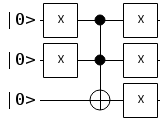
\includegraphics[scale=0.6]{OR.png}
    \caption{Representation of OR gate using 1 Toffoli gate and 5 NOT gates}
    \label{fig:awesome_image}
\end{figure} 

For every AND and every OR in the classical circuit we are given, we will need one extra qubit. The extra qubit is always the third bit for the Toffoli gate. We now have every part to simulate the classical circuit on the quantum circuit. However, this is not yet our oracle.

At this point, we have a ciruit takes the input $\left | x \right \rangle \left | 0^{k} \right \rangle$ and gives $\left | junk(x) \right \rangle \left | f(x) \right \rangle$. However, we need it to be of the form \cite{kothari12} 

$$\left | x \right \rangle \left | q \right \rangle \to \left | x \right \rangle \left | f(x) \oplus q \right \rangle$$

What this means is that we need to preserve the state of $\left | x \right \rangle$ through the circuit. Though this wouldn't be possible on a classical computer, we can use a handy little trick called ``uncomputation" for the quantum ciruit. Because every quantum gate is reversible, to get $\left | x \right \rangle$ back, we just have to perform all our gates in backward order. However, before we do that, we copy the result of the search function onto a new qubit using a CNOT gate. Then we can perform the uncomputation on the rest of the qubits, resulting in the desired form for the output.

At this point, the general steps for our algorithm are:

\begin{enumerate}
	\item Given an input function in the form of a classical circuit, we simulate each classical gate with a quantum gate, taking note of the order and which qubits we applied the gates to.
	\item Copy the output of the function, which should be the state of $nth$ qubit, to an extra qubit.
	\item Perform the uncomputation by applying the same quantum gates we applied before but in the opposite order. 
\end{enumerate}

After we have achieved this circuit, we then need to complete the final step necessary for the oracle. By definition, the oracle flips the phase of the system state for a single input. This means that if the output qubit is in the $\left | 1 \right \rangle$ state, then we want to flip the phase of the entire system state. This can be done with one more extra qubit and a Pauli-Z gate with a control on the ouput qubit.

However, we still have one final problem: the output qubit needs to be returned to its original state from before the oracle. The simplest way to return it to its original state is performing the simulated classical circuit once again. After this, we have will a quantum circuit that fully implements the oracle for Grover's algorithm.

\begin{figure}[H]
\begin{framed}
\textbf{To construct a circuit that implements the oracle for Grover's algorithm:}
\begin{enumerate}
\item Obtain a classical circuit, called $C_{c}$ that implements the desired search function using AND, OR and NOT gates.
\item Using quantum NOT and Toffoli gates, simulate the classical circuit with a quantum one, called $C_{q}$. (Note: for $N=n^{2}$ possible solutions to the search function, and $g$ classical gates, this quantum circuit will require $n+g$ qubits.)
\item Copy the output of this circuit to another qubit (called the output qubit) by using a quantum controlled NOT gate.
\item Using one more qubit, perform a Pauli-Z gate on this extra qubit with a control on the output qubit. Note that the oracle function will require a total of $n+g+2=n_{q}$ qubits.
\item Apply $C_{q}$ again to return the output qubit back to its original state.
\end{enumerate}
\end{framed}
\end{figure}



\section{Conclusion}

By representing a quantum computer as a series of matrix operations, I was able to successfully simulate qubits as well as perform Grover's algorithm. Furthermore, I was able to write code that represents performing the necessary quantum operations for the oracle function.

\begin{thebibliography}{9}

	\bibitem{grover96}
	Grover, L. K. (1996, July). A fast quantum mechanical algorithm for database search. \emph{In Proceedings of the twenty-eighth annual ACM symposium on Theory of computing} (pp. 212-219). ACM.
  
	\bibitem{rojas04}
  Rojas, R. (2004). A tutorial introduction to the lambda calculus. DOI= http://www.utdallas.edu/\textasciitilde gupta/courses/apl/lambda.pdf.
  
  \bibitem{tonder04}
  Van Tonder, A. (2004). A lambda calculus for quantum computation. \emph{SIAM Journal on Computing}, 33(5), 1109-1135.
  
  \bibitem{spector04}
  Spector, L. (2004). Automatic Quantum Computer Programming: a genetic programming approach (Vol. 7). \emph{Springer Science and Business Media}.
  
  \bibitem{kothari12}
  http://mathoverflow.net/questions/102779/how-much-does-a-quantum-oracle-to-find-a-needle-in-a-haystack-really-cost

\end{thebibliography}


\end{document}
